\section{梯度下降}
损失函数的优化求解可以通过梯度下降法实现,对于以下参数优化:
\begin{equation}
\theta^* = \arg \min L(\theta)
\end{equation}
其中,$L$为损失函数,$\theta$为优化参数。使用梯度下降迭代求解:
\begin{equation}
	\theta_n = \theta_{n-1} - \left. \eta \frac{\partial L)}{\partial \theta}\right|_{\theta_{n-1}}
\end{equation}

\subsection{学习率微调}
学习率$\eta$的调整是梯度下降法中重要的一环,过大、过小的学习率影响迭代求解的收敛性和效率。太小的学习率导致算法收敛太慢,过大的学习率反而导致算法发散,具体形象的描述可见图\ref{fig:learning_rate}。
\begin{figure}
	\centering
	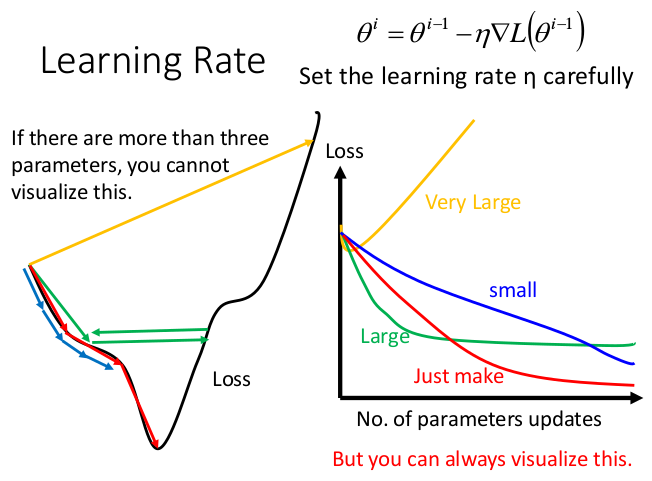
\includegraphics[scale=0.4]{pic/learning_rate}
	\caption{不同学习率下的算法迭代情况}
	\label{fig:learning_rate}
\end{figure}

通常情况下需要随着迭代次数的增加,逐渐减小学习率,主要原因是,学习的初始阶段,距离目标较远,损失函数很大,需要大的学习率,经过多轮迭代后,逐渐接近目标点,此时可以缩小学习率。

一个简单的自适应学习率可以设置为$\frac{\eta}{\sqrt{t+1}}$。

\subsubsection{adagrad}
adagrad 的权值参数设置为所有以往迭代时微分值的均方根值。权重$w$梯度表示为:
\begin{align}
g^t &= \frac{\partial (\theta^t)}{\partial w}\\
w^{t+1} &= w^t - \frac{\eta^t}{\sigma^t}g^t\\
  \\
\sigma^t &= \sqrt{\frac{1}{t+1}\sum_{i=0}^{t}(g^i)^2}
\end{align}
当$\eta^t = \frac{\eta}{\sqrt{t+1}}$时,
\begin{equation}
w^{t+1} = w^t - \frac{\eta}{\sigma^t}g^t = \frac{\eta}{\sqrt{\sum_{i=0}^{t}(g^i)^2}}
\end{equation}
\begin{myquotation}{adagrad中的疑问}
	当有大的梯度时,$g^t$导致大的步长,但分母$\sigma ^ t$导致小的步长,是否矛盾?
\end{myquotation}

\subsection{随机梯度下降法 Stochastic Gradient Descent}

\subsection{特征缩放}

\subsection{梯度下降数学理论}



